\documentclass[runningheads]{comsis2}

%% Necessary definitions for the running heads
\def\journalissue{Computer Science and Information Systems 00(0):0000--0000}
\def\paperidnum{https://doi.org/10.2298/CSIS123456789X}
\setcounter{page}{1}

%% Use this to show line numbers (and remove only in the final camera-ready version)
\usepackage[pagewise]{lineno}
\linenumbers
\usepackage{hyperref}
\usepackage{verbatim}
\usepackage{graphicx}
\usepackage{amsmath}
\usepackage[normalem]{ulem}


%%%%% NEW PACKAGES 
\usepackage{graphicx}
\usepackage{color, colortbl}
\graphicspath{ {./figures/} }

\newcommand*{\Comb}[2]{{}C^{#1}_{#2}}%
%%%%%%%

\title{Logical dependencies: extraction from the versioning system and an example of usage
\footnote{If this is an extended version of a conference paper, it should be clearly stated here.}}

%% Use this if the title is too long for the running heads
\titlerunning{Logical dependencies in practice}

\author{Adelina Diana Stana\inst{1} \and Ioana Şora\inst{2}}

%% Use this the list of authors is too long for the running heads
%\authorrunning{First Author et al.}

\institute{Stana Adelina Diana\\
  Politehnica University, Piaţa Victoriei Nr. 2, ; 300006 Timişoara, jud. Timiş, România\\
  \email{stana.adelina.diana@gmail.com}
  \and
  Şora Ioana\\
 Politehnica University, Piaţa Victoriei Nr. 2, ; 300006 Timişoara, jud. Timiş, România\\
  \email{ioana.sora@cs.upt.ro}}

\begin{document}

\maketitle

\begin{abstract}
The version control system of every software product can provide important information about how the system is connected. 
In this study, we first propose a language-independent method to collect and filter dependencies from the version control, and second, we use the results obtained in the first step to identify key classes from three software systems. To identify the key classes, we are using the dependencies extracted from the version control system together with dependencies from the source code, but also separate. Based on the results obtained we can say that, compared with the results obtained by using only dependencies extracted from code, the mix between both types of dependencies do not provide dramatically different results, only small improvements. And, by using only dependencies from the version control system, we obtained results that did not surpass the results previously mentioned, but are still acceptable.
Even though the logical dependencies results are only acceptable, this might open an important opportunity for software systems that use dynamically typed languages such as JavaScript, Objective-C, Python, Ruby, or systems that use multiple languages. These types of systems, for which the code dependencies are harder to obtain, can use the dependencies extracted from the version control to gain better knowledge about the system.
  
\vspace{6pt}\textbf{Keywords:} logical dependencies; logical coupling; mining software repositories; versioning system; key classes; co-changing entities; software evolution.
\end{abstract}


\section{Introduction}



The version control ( also known as source control ) system that tracks changes in source code during software development can provide useful information about the system's details. 
The usage of information extracted from the version control system is not something new, previous works have used version control information to detect design issues \cite{Zimmermann:2004:MVH:998675.999460}, predict fault incidence among modules \cite{Predictingfaultincidence}, \cite{Cataldo2009SoftwareDW} or guide software changes \cite{4815274}, \cite{DBLP:journals/ese/AjienkaCC18}.
In software engineering literature, concepts like evolutionary coupling, evolutionary dependencies, logical dependencies, or logical coupling refer to the same sort of relationship among software entities. That relationship is extracted from the version control system and can mean that the entities from the source code files that are changing together, evolve together, and might depend on one another. Studies show that dependency relationships found in the source code overlap only in a small percentage with dependency relationships found in the version control system, and suggest that these two types of relationships can be used together \cite{Oliva:2011:ISL:2067853.2068086}, \cite{DBLP:journals/jss/AjienkaC17}. But, in practice, dependencies extracted from the version management system are rarely used due to the size of the information extracted \cite{Shtern:2012:CMS:2332427.2332428}. A relatively small source code repository with roundabout one thousand commits can lead to millions of connections. 
In this paper, we intend to speed up the processing time, reduce the size of connections extracted from the version control and, increase the confidence that the connections obtained might be related by applying a set of filters with different thresholds to the information extracted. 
In order to validate the results obtained, and to see if the filtering methods had or not had a favorable effect on the final result, we want to identify the key classes of different systems. The identification of key classes had been previously performed by using structural dependencies, so,
we intend to use the results obtained together with structural dependencies, and also separate, and see how the final results fluctuate.

The paper is organized as follows: Section 2 introduces the concepts of logical dependencies and the methods of obtaining them. Section 3 introduces the concept of key classes and the new approach of using logical dependencies to detect key classes. Section 4 defines the data set used, and presents the new results obtained with the data set. Finally, section 5 discusses the conclusions based on the results obtained. 




\section{The concept of logical dependencies}

\subsection{State of the art}

The concept of logical coupling (dependency) was first introduced by Gall et al. \cite{Gall:1998:DLC:850947.853338}. They defined the logical dependency between two software entities (classes, modules, interfaces, etc. ) as the fact that the entities repeatedly change together during the historical evolution of a software system.
Since then, logical dependencies have been used in multiple areas of software engineering, most commonly in fault and change prediction.  
Besides the studies on how logical dependencies can help gain knowledge about software systems, some studies also focused on the interplay between logical and structural dependencies. Ajienka et al. and Olivia et al. studied the interplay between structural and logical dependencies, and they concluded that, in most cases, structural dependencies do not lead to logical dependencies \cite{Oliva:2011:ISL:2067853.2068086}, \cite{DBLP:conf/issre/OlivaG15}, \cite{DBLP:journals/jss/AjienkaC17}. The above affirmation is also supported by Lanza et al., who consider that logical dependencies are important because they can reveal dependencies that are not visible via code analysis \cite{inproceedings_radar_evolution}.



In previous research, the \textit{support} and \textit{confidence} metrics were used to measure the strength of a logical dependency. 
The logical dependencies are commonly represented as directed association rules, the association rule between A and B ( $A \rightarrow B$) means that changes in entity A cause changes in entity B, where A is the antecedent, and B is the consequent of the rule. 
The support metric counts the number of commits in which both entities of an association rule change together. The confidence metric is the ratio between the support metric and the total number of commits in which the antecedent of the rule was involved. 

By appling different thresholds to the metrics presented above, the logical dependencies to further use where selected \cite{DBLP:conf/issre/OlivaG15}, \cite{DBLP:journals/jss/AjienkaC17}, \cite{Zimmermann:2004:MVH:998675.999460}.


\subsection{Current approach}


To avoid confusion, we call \textit{co-changing pairs} all the association rules of one system. The association rules are formed between two software entities that update together in the same commit.
For example, a commit that contains seven entities will generate 21 co-changing pairs ($\Comb{n}{k}=\frac{n!}{k!(n-k)!} = \frac{7!}{2!(5)!} = 21$).


The \textit{logical dependencies} are the association rules whose metrics fulfill certain conditions. So, the logical dependencies are a subset of the co-changing pairs. 

The conditions that need to be met by a co-changing pair to be considered a logical dependency are called \textit{filters}. Like in other research regarding logical dependencies, our filters are thresholds applied to the metrics of association rules. 

Previously, we tried to filter logical dependencies from co-changing pairs by applying filters like the occurrence filter and commit size filter \cite{saci19}, \cite{enase19}. 
The commit size filter, presented in more detail in section \ref{commit_filter}, and used by other authors \cite{DBLP:journals/jss/AjienkaC17}, proved to be helpful, and it will be also used for this paper. 
But, we cannot say the same for the occurrence filter, the filter consisted of different thresholds applied to the support metric and proved to not work well for systems with few commits.

So currently, we aim to refine the filtering method with a new filter that can be applied for all sorts of commit history sizes. This new filter, presented in section \ref{strength_filter}, will be used together with the commit size filter to filter logical dependencies from co-changing pairs. The entire process of extracting co-changing pairs from the versioning system, filtering them to obtain logical dependencies, and exporting the results is done with a tool written in Python. The workflow is presented in figure \ref{fig:workflow_key}.

\begin{figure}
\centering
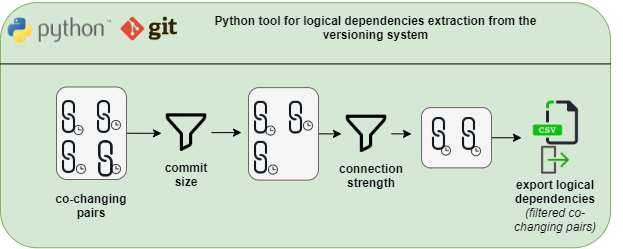
\includegraphics[width=\textwidth]{ld_workflow.png}
\caption{Workflow for logical dependencies extraction.}
\label{fig:workflow_key}
\centering
\end{figure}

\subsection{Commit size filter}
\label{commit_filter}

The commit size filter filters out all co-changing pairs from commits with more than 10 files changed. We consider that commits with more than 10 files changed tend to be code unrelated; we studied the commit size trend from serval git open-source repositories, and we concluded that most of the commits contain less than ten files. On average, only 10 \% of the total commits have more than ten files changed. 

This filter will also prevent the volume of data processed from going out of proportion. In some of the repositories studied, we found commits with more than 1000 files; these commits could generate over half a million co-changing pairs if the commit size filter is not applied. 



\subsection{Connection strength filter}
\label{strength_filter}


The connection strength filter is new for our research regarding logical dependencies identification, and it is based on our experience with the occurrence filter.
An important conclusion drawn from the results obtained with the occurrence filter is that setting a hard threshold for a filter is not always a good idea. A certain threshold can work well with a medium/large-sized system but, when applied to a small-sized system, can reduce the co-changes filtered to 0. To avoid this type of situation, we evaluated a filter that considers the system's specifications. 


As we previously mentioned, a filter has two components: the metrics computed for each co-changing pair (association rule) and the threshold values. The connection strength filter's metrics derive from the support and the confidence metric.

For an association rule (co-changing pair) formed from the ascendent A and consequent B ($A \rightarrow B$), 
the support count is the total number of commits in which both entities are involved,


$support (A \rightarrow B) = freq_{total\ commits} {(A \cup B)}$

and the confidence is the ratio between the support and the frequency of the ascendent of the rule.

$confidence (A \rightarrow B) =\frac{support (A \rightarrow B) }{freq_{total\ commits}(A)}$

The only problem with the confidence metric, as it is defined above, is that it does not include the big picture of the system.
The best value for the confidence metric is 1, meaning that in all commits in which entity A is present, entity B is also there. If, for example, we have a co-changing pair $A \rightarrow B$, and A updates only once in the entire history, and in that time, updates together with B, then the confidence metric associated with the co-changing pair will be 1 (the best value possible). That is not a fair value compared with other scenarios. For example, we can have the co-changing pair $A \rightarrow B$, and A updates 100 in the entire history from which 80 times updates together with B, leading to a confidence value of 0.8.
Even though in the second scenario we have a confidence value smaller than in the first scenario, the second scenario could lead to a more trustworthy connection.


Figures \ref{fig:strength_overview_ant} and \ref{fig:strength_overview_hibernate}  intend to offer the big picture of two systems, one small-sized (Ant) and one medium-sized(Hibernate). In both figures, the dots represent the maximum number of updates of one entity with another, and the blue line represents the average occurrence value of the system.
It can be observed that both systems have multiple entities that update only once (the dark line at the bottom), meaning that we might have many confidence values of 1 (highest value possible) for entities that update only once together.

To consider also the big picture of the system, we defined a new metric for a co-changing pair (association rule), called the connection strength metric. The metric considers the mean value of all the occurrences between two entities from the system. Also, the values obtained are clipped between 0 and 100, where 100 is the best value to obtain and 0 is the worst.


$ system factor for (A \rightarrow B) =\frac{support (A \rightarrow B) }{system\ mean}$

$ strength (A \rightarrow B) =\frac{support (A \rightarrow B) * 100}{freq_{total\ commits}(A)} * system\ factor$

By using the strength metric, if we consider again the two scenarios presented above, and a system mean value of 10, we will have the following values: for the scenario in which entity A and B update only once, and in that one update, update together, the strength metric value is 10. For the scenario in which entity A updates 100 in the entire history from which 80 times updates together with B, the strength metric value is 100.  

\begin{figure}
\centering
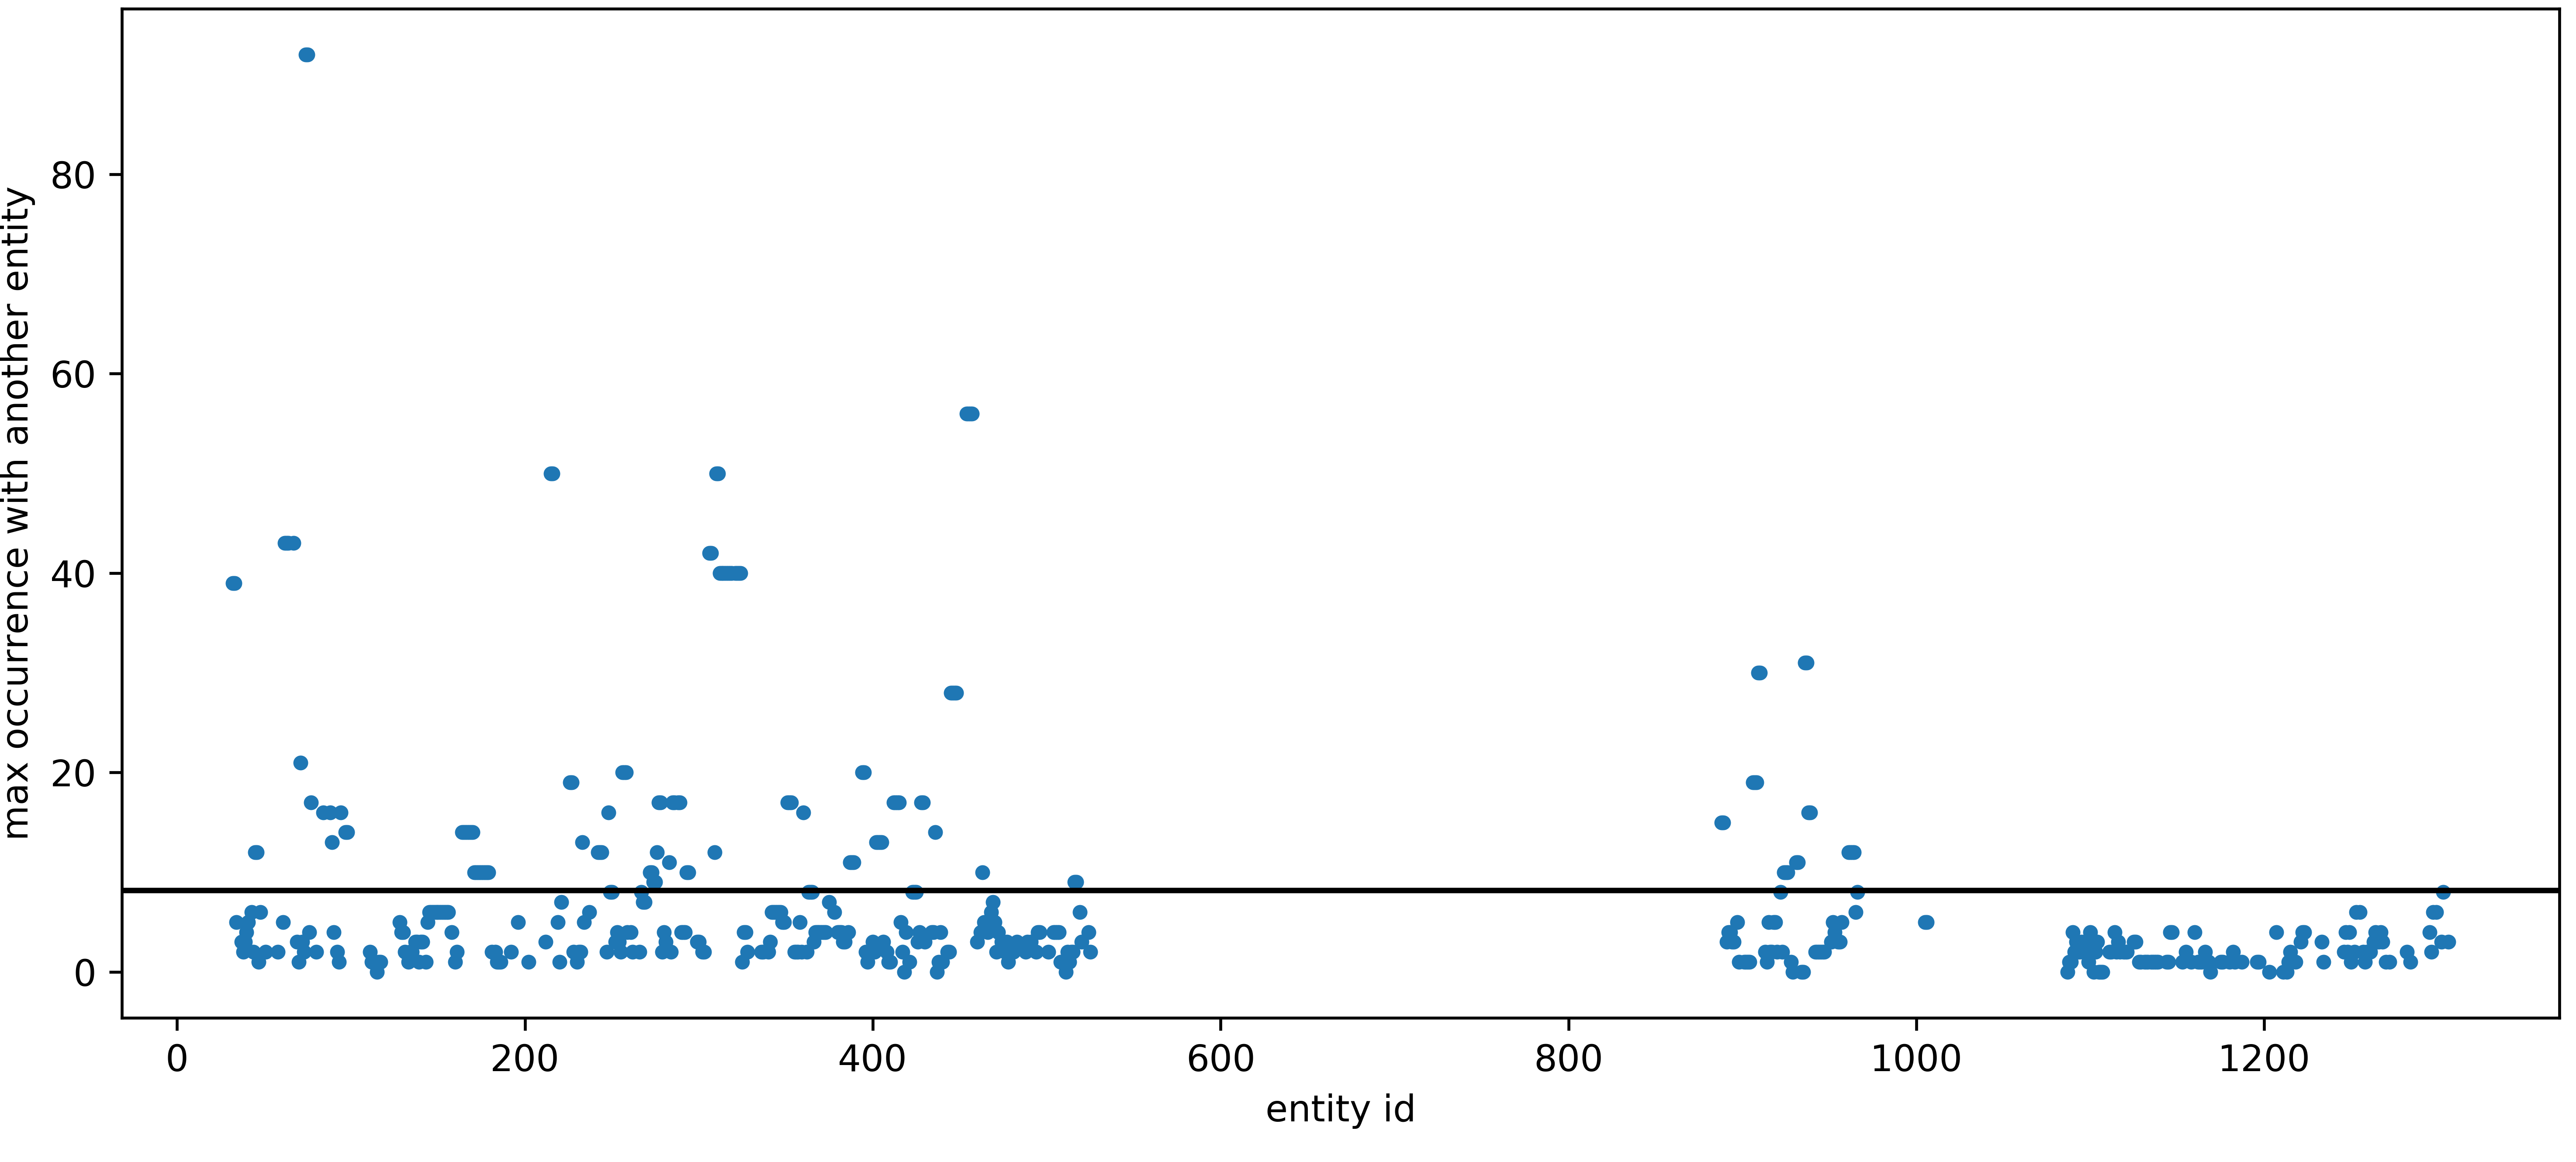
\includegraphics[scale=0.7]{fig_ant_maxOcc.png}
\caption{Overview of the number of occurences in Ant. }
\label{fig:strength_overview_ant}
\centering
\end{figure}

\begin{figure}
\centering
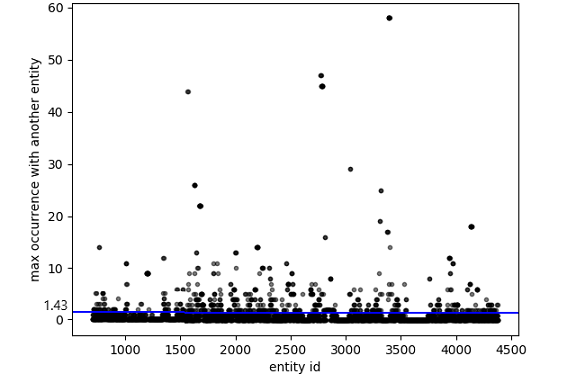
\includegraphics[scale=0.7]{fig_hibernate_maxOcc.png}
\caption{Overview of the number of occurences in Hibernate. }
\label{fig:strength_overview_hibernate}
\centering
\end{figure}


Since the values can vary from 0 to 100, the filter threshold values begin at 10 and are incremented by 10, until 100. We do not settle for one value because we want to see how the threshold values affect the number of remaining co-changing pairs and the output of their usage.

In figure \ref{fig:strength_overview} we plotted the number of structural dependencies, co-changing pairs before filtering, and co-changing pairs after filtering for two systems, one small-sized and one medium-sized. With the connection strength filter, the small-sized system didn't lose all the co-changing pairs once with the filtering.

\begin{figure}
\centering
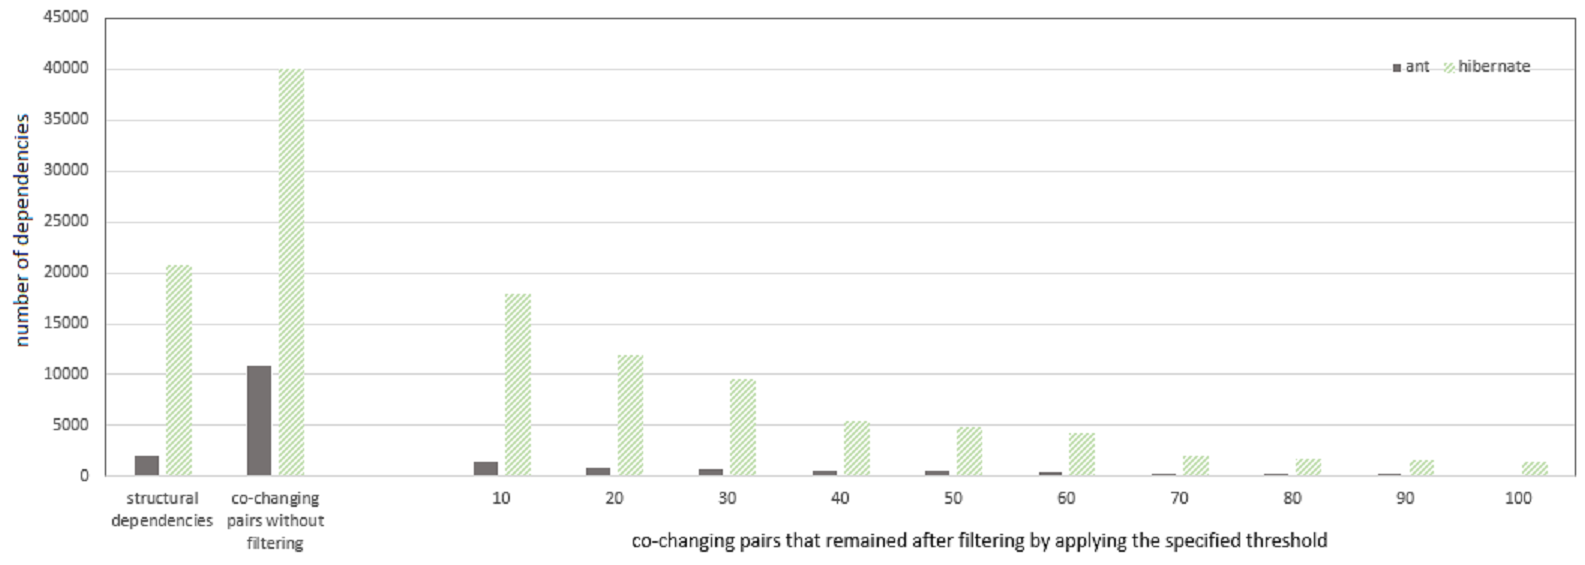
\includegraphics[width=\textwidth]{strength_overview.PNG}
\caption{Overview of the impact of connection strength filtering on the number of co-changing pairs. }
\label{fig:strength_overview}
\centering
\end{figure}


We compare the number of remaining co-changing pairs with the number of structural dependencies because according to surveys \cite{Shtern:2012:CMS:2332427.2332428}, \cite{sar}, the main reason why logical dependencies (filtered co-changes) are not used together with structural dependencies is because of their size. So, it is essential to get an overview of the comparison between the co-changing pairs number and the structural dependencies number at each filtering step.

We call the co-changing pairs that remain after filtering, logical dependencies. 

After this step, we will use the logical dependencies obtained with different threshold values and see which threshold value performs the best. Up until now, we only looked at the size of the resulting logical dependencies and decided if a filter and its threshold are good or not. Now, we can also look at the results obtained by using the logical dependencies and decide.

\section{Key classes: baseline versus current approach}
\label{sec:baseline_approach}

\subsection{State of the art}

Zaidman et al \cite{ZaidmanJurnal} were the first to introduce the concept of key classes and it refers to classes that can be found in documents written to provide an architectural overview of the system or an introduction to the system structure. 
Tahvildari and Kontogiannis have a more detailed definition regarding key classes concept: “Usually, the most important concepts of a system are implemented by very few key classes which can be characterized by the specific properties. These classes, which we refer to as key classes, manage many other classes or use them in order to implement their functionality. The key classes are tightly coupled with other parts of the system. Additionally, they tend to be rather complex, since they implement much of the legacy system’s functionality” \cite{Tahvildari2004ImprovingDQ}.


The key class identification can be done by using different algorithms with different inputs. In the research of Osman et al., the key class identification is made by using a machine learning algorithm and class diagrams as input for the algorithm \cite{6676885}. Thung et al. builds on top of Osman et al.’s approach and adds network metrics and optimistic classification in order to detect key classes \cite{rocclasification}.  

Zaidman et al. use a webmining algorithm and dynamic analysis of the source code to identify the key classes \cite{ZaidmanJurnal}.

\subsection{Baseline approach}
We use the research of I. Şora et al \cite{Finding-key-classes} as a baseline for our research involving the usage of logical dependencies to find key classes. 

Şora et al. used the static analysis of the source code, a page ranking algorithm and other class attributes to find key classes \cite{PagerankENASE}, \cite{enase15}, \cite{SoraSpringer}, \cite{PagerankSACI},\cite{Finding-key-classes}.
The page ranking algorithm is a customization of PageRank, the algorithm used to rank web pages \cite{ilprints422} and works based on a recommendation system. If one node has a connection with another node, then it recommends the second node. In previous works, connections are established based on structural dependencies extracted from static code analysis. If A has a structural dependency with B, then A recommends B, and also B recommends A.

The ranking algorithm ranks all the classes from the source code of the system analyzed according to their importance. To identify the important classes from the rest of the classes a threshold for TOP classes from the top of the ranking is set. The TOP threshold value can go from 1 to the total number of classes found in the system. 



\subsection{Current approach}

The baseline approach uses a tool that takes as an input the source code of the system and applies ranking strategies to rank the classes according to their importance. We modified the tool used by the baseline approach to take also the logical dependencies as input; the rest of the workflow is the same as in the baseline approach ( figure \ref{fig:baseline_approach} ).

\begin{figure}
\centering
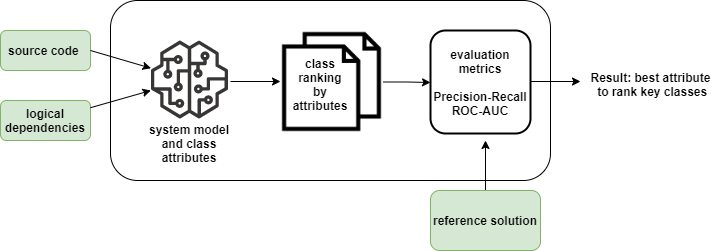
\includegraphics[width=\textwidth]{current_approach.PNG}
\caption{Overview of the current approach.}
\label{fig:baseline_approach}
\centering
\end{figure}

In order to rank the classes according to their importance, different class metrics are used \cite{Ding2016AnIA}, \cite{ZaidmanJurnal}, \cite{PAN2018188}. Below are some of the class metrics used in the baseline approach and our current research to rank the classes according to their importance. We use only a subset of the metrics used in previous research because the extracted logical dependencies are undirected.


The class metrics used can be separated into two categories: class connection metrics and class PageRank values.
The class connection metrics are CONN-TOTAL-W, which is the total weight of all connections of the class, and CONN-TOTAL, the total number of distinct classes that a class uses or are used by a class \cite{Finding-key-classes}.

Previous research used PageRank values computed on both directed and undirected, weighted and unweighted graphs. In the current research, we used the PR, which is the PageRank value computed on the directed and unweighted graph. The PR-U, which is the value computed on the undirected and unweighted graph, and PR-U2-W, the value computed on the weighted graph with back-recommendations \cite{PagerankENASE}, \cite{enase15}, \cite{Finding-key-classes}, \cite{PagerankSACI}.




\subsection{Metrics for results evaluation}
\label{sec:evalmetrics}
To evaluate the quality of the key classes ranking algorithm and solution produced, the key classes found by the algorithm are compared with a reference solution. The reference solution is extracted from the developer documentation.  Classes mentioned in the documentation are considered key classes and form the reference solution (ground truth) used for validation \cite{7551990}. 

For the comparison between both solutions, a classification model is used. The quality of the solution produced is evaluated by using the Receiver Operating Characteristic Area Under Curve (ROC-AUC) metric, a metric that evaluates the performance of a classification model.


\textit{Receiver Operating Characteristic Area Under Curve}


The ROC graph is a two-dimensional graph that has on the X-axis plotted the false positive rate and on the Y-axis the true positive rate. By plotting the true positive rate and the false positive rate at thresholds that vary between a minimum and a maximum possible value we obtain the ROC curve. The area under the ROC curve is called Area Under the Curve (AUC).

The true positive rate of a classifier is calculated as the division between the number of true positive results identified and all the positive results identified:

\begin{equation}
 True\ positive\ rate (TPR) = \frac{TP}{TP+FN}
\end{equation}
The false positive rate of a classifier is calculated as the division between the number of false positive results identified and all the negative results identified:

\begin{equation}
 False\ positive\ rate (FPR) = \frac{FP}{FP+TN}
\end{equation}

The true positives (TP) are the classes found in the reference solution and also in the top TOP ranked classes. False positives (FP) are the classes that are not in the reference solution but are in the TOP ranked classes.
True Negatives (TN) are classes that are found neither in the reference solution nor in the TOP ranked classes. False Negatives (FN) are classes that are found in the reference solution but not found in the TOP ranked classes.

In multiple related works, the ROC-AUC metric has been used to evaluate the results for finding key classes of software systems.
For a classifier to be considered good, its ROC-AUC metric value should be as close to 1 as possible, when the value is 1 then the classifier is considered to be perfect.

Osman et al. obtained in their research an average Area Under the Receiver Operating Characteristic Curve (ROC-AUC) score of 0.750 \cite{6676885}. Thung et al. obtained an average ROC-AUC score of 0.825 \cite{rocclasification}  and Şora et al. (the baseline) obtained an average ROC-AUC score of 0.894 \cite{Finding-key-classes}.



\section{Experimental results using logical dependencies}
\label{sec:current_measurements}

As we mentioned in the beginning the purpose is to check if the logical dependencies can improve key class detection. 

As presented in section \ref{sec:baseline_approach}, the key class detection was done by using structural dependencies of the system. 
In this section, we will use the same tool used in the baseline approach presented in section \ref{sec:baseline_approach}, and we will add a new input to it, the logical dependencies. 

Below is a comparison between the new approach and baseline approach, how we collect the logical dependencies, the results obtained previously, and the new results obtained. 
The new results are separated into two categories, the results obtained by using structural and logical dependencies and the results obtained by using only logical dependencies. 

\subsection{Data set used}
\label{sec:dataset}
In this section, we will look over all the systems studied in the baseline research presented in section \ref{sec:baseline_approach}, and we will try to identify the systems that could be used also in our current research involving logical dependencies.


The research of I. Sora et al \cite{Finding-key-classes} takes into consideration structural public dependencies that are extracted using static analysis techniques and was performed on the object-oriented systems presented in table \ref{tab:gitfoundsystems}.

The requirements for a system to qualify as suited for investigations using logical dependencies are: has to be on GitHub, has to have releases to identify a specific version (previous research was done only on specific releases), and also, has to have a significant number of commits. 
From the total of 14 object-oriented systems listed in the paper \cite{Finding-key-classes}, 13 of them have repositories in Github \ref{tab:gitfoundsystems}. And from the found repositories, only 6 repositories have the same release tag as the specified version in previous research.
The commits number found on the remaining 6 repositories varies from 19108 commits for Tomcat Catalina to 149 commits for JHotDraw. In order to have more accurate results, we need a significant number of commits, so we reached the conclusion that only 3 systems can be used for key classes detection using logical dependencies: Apache Ant, Hibernate, and Tomcat Catalina.  From all the systems mentioned in table \ref{tab:gitfoundsystems} Apache Ant is the most used and analyzed in other  works \cite{enase19}, \cite{7332515}, \cite{1402122}, \cite{Kamran2016IdentificationOC}.

\begin{table}
\renewcommand{\arraystretch}{1}
\caption{Found systems and versions of the systems in GitHub. }
\label{tab:gitfoundsystems}
\centering
\begin{tabular}{lllll}
\hline
ID	&	System	&	Version	&	Release Tag name	&	Commits number	\\
\hline
Sl	&	Apache Ant	&	1.6.1	&	rel/1.6.1	&	6713	\\
S2	&	Argo UML	&	0.9.5	&	not found	&	0	\\
S3	&	GWT Portlets	&	0.9.5 beta	&	not found	&	0	\\
S4	&	Hibernate 	&	5.2.12	&	5.2.12	&	6733	\\
S5	&	javaclient	&	2.0.0	&	not found	&	0	\\
S6	&	jEdit	&	5.1.0	&	not found	&	0	\\
S7	&	JGAP	&	3.6.3	&	not found	&	0	\\
S8	&	JHotDraw	&	6.0b.1	&	not found	&	149	\\
S9	&	JMeter	&	2.0.1	&	v2\_1\_1	&	2506	\\
S10	&	Log4j	&	2.10.0	&	v1\_2\_10-recalled	&	634	\\
S11	&	Mars	&	3.06.0	&	not found	&	0	\\
S12	&	Maze	&	1.0.0	&	not found	&	0	\\
S13	&	Neuroph	&	2.2.0	&	not found	&	0	\\
S14	&	Tomcat Catalina	&	9.0.4	&	9.0.4	&	19108	\\
S15	&	Wro4J	&	1.6.3	&	v1.6.3	&	2871	\\
\hline
\end{tabular}
\end{table}





\subsection{Measurements using only the baseline approach}


In table \ref{tab:previousresults} are presented the ROC-AUC values for different attributes computed for the systems Ant, Tomcat Catalina, and Hibernate by using the baseline approach. We intend to compare these values with the new values obtained by using also logical dependencies in key class detection.

\begin{table}[!h]
\renewcommand{\arraystretch}{1}
\caption{ROC-AUC metric values extracted. }
\label{tab:previousresults}
\centering
\scalebox{0.9}{
\begin{tabular}{|c|ccc|}
\hline
Metrics &	Ant	&	Tomcat Catalina	&	Hibernate	\\
\hline

PR\_U2\_W	&	0.95823	&	0.92341	&	0.95823	\\
PR	&	0.94944	&	0.92670	&	0.94944	\\
PR\_U	&	0.95060	&	0.93220	&	0.95060	\\
CONN\_TOTAL\_W	&	0.94437	&	0.92595	&	0.94437	\\
CONN\_TOTAL	&	0.94630	&	0.93903	&	0.94630	\\

\hline
\end{tabular}
}
\end{table}





\subsection{Measurements using combined structural and logical dependencies}

The tool used in the baseline approach runs a graph-ranking algorithm. 
The graph used contains the structural dependencies extracted from static source code analysis.
Each edge in the graph represents a dependency, the entities that form a structural dependency are represented as vertices in the graph. 
As mentioned in section \ref{sec:baseline_approach}, we modified the tool to read also logical dependencies and add them to the graph. 
In this section, we add in the graph the logical dependencies together with the structural dependencies. 

In tables \ref{tab:measurementscombined:ant}, \ref{tab:measurementscombined:tomcat}, and \ref{tab:measurementscombined:hibernate}, on each line, we have the metric that is calculated and on each column, we have the connection strength threshold that was applied to the logical dependencies used in identifying the key classes.
We started with logical dependencies that have a connection strength greater than 10\%, which means that in at least 10\% of the commits involving A or B, A and B update together. Then we increased the threshold value by 10 until we remained only with entities that update in all the commits together. The last column contains the results obtained previously by the tool by only using structural dependencies.

As for the new results obtained by combining structural and logical dependencies, the values close to the previously registered values, but did not surpass them, are underlined with one line. And, with two lines, are underlined the values that are better than the previously registered values. At this step, we can also observe that for all three systems measured in tables \ref{tab:measurementscombined:ant}, \ref{tab:measurementscombined:tomcat}, and \ref{tab:measurementscombined:hibernate}, the best values obtained are for connection strength between 40-70\%.

\begin{table}[!h]
\setlength\tabcolsep{3.5pt}
\caption{Measurements for Ant using structural and logical dependencies combined}
\label{tab:measurementscombined:ant}
\centering
\begin{tabular}{|c|cccccccccc|c|}
\hline
Metrics &	$\geq10$	&	$\geq20$		&	$\geq30$		&	$\geq40$		&	$\geq50$		&	$\geq60$		&	$\geq70$		&	$\geq80$		&	$\geq90$		&	$\geq100$		&	Baseline \\
\hline

PR\_U2\_W	&	0.877	&	0.880	&	0.883	&	0.888	&	0.884	&	0.880	&	0.901	&	0.924	&	0.900	&	0.891	&	0.929	\\
PR	&	0.955	&	0.932	&	0.936	&	0.936	&	0.880	&	0.884	&	0.887	&	0.889	&	0.888	&	0.890	&	0.855	\\
PR\_U	&	0.933	&	0.937	&	0.936	&	0.939	&	0.940	&	0.939	&	0.941	&	0.943	&	0.942	&	0.940	&	0.933	\\
CON\_T\_W	&	0.841	&	0.839	&	0.836	&	0.838	&	0.835	&	0.849	&	0.859	&	0.872	&	0.870	&	0.874	&	0.934	\\
CON\_T	&	0.920	&	0.919	&	0.921	&	0.923	&	0.923	&	0.932	&	0.934	&	0.939	&	0.937	&	0.937	&	0.942	\\

\hline
\end{tabular}
\end{table}


\begin{table}[!h]
\setlength\tabcolsep{3.5pt}
\caption{Measurements for Tomcat using structural and logical dependencies combined}
\label{tab:measurementscombined:tomcat}
\centering
\begin{tabular}{|c|cccccccccc|c|}
\hline
Metrics &	$\geq10$	&	$\geq20$		&	$\geq30$		&	$\geq40$		&	$\geq50$		&	$\geq60$		&	$\geq70$		&	$\geq80$		&	$\geq90$		&	$\geq100$		&	Baseline \\
\hline

PR\_U2\_W	&	0.862	&	0.883	&	0.898	&	0.901	&	0.907	&	0.909	&	0.910	&	0.916	&	0.918	&	0.918	&	0.923	\\
PR	&	0.879	&	0.885	&	0.888	&	0.882	&	0.869	&	0.869	&	0.863	&	0.863	&	0.863	&	0.863	&	0.927	\\
PR\_U	&	0.924	&	0.930	&	0.931	&	0.932	&	0.932	&	0.932	&	0.932	&	0.932	&	0.932	&	0.932	&	0.932	\\
CON\_T\_W	&	0.868	&	0.888	&	0.901	&	0.909	&	0.914	&	0.917	&	0.918	&	0.923	&	0.925	&	0.925	&	0.926	\\
CON\_T	&	0.925	&	0.934	&	0.937	&	0.938	&	0.938	&	0.938	&	0.938	&	0.938	&	0.938	&	0.938	&	0.939	\\
																										

\hline
\end{tabular}
\end{table}


\begin{table}[!h]
\setlength\tabcolsep{3.5pt}
\caption{Measurements for Hibernate using structural and logical dependencies combined}
\label{tab:measurementscombined:hibernate}
\centering
\begin{tabular}{|c|cccccccccc|c|}
\hline
Metrics &	$\geq10$	&	$\geq20$		&	$\geq30$		&	$\geq40$		&	$\geq50$		&	$\geq60$		&	$\geq70$		&	$\geq80$		&	$\geq90$		&	$\geq100$		&	Baseline \\
\hline

PR\_U2\_W	&	0.903	&	0.909	&	0.916	&	0.928	&	0.930	&	0.932	&	0.946	&	0.947	&	0.947	&	0.949	&	0.958	\\
PR	&	0.956	&	0.959	&	0.961	&	0.962	&	0.962	&	0.962	&	0.953	&	0.953	&	0.953	&	0.954	&	0.949	\\
PR\_U	&	0.937	&	0.941	&	0.943	&	0.947	&	0.948	&	0.948	&	0.950	&	0.950	&	0.950	&	0.950	&	0.951	\\
CON\_T\_W	&	0.864	&	0.872	&	0.879	&	0.896	&	0.898	&	0.900	&	0.929	&	0.930	&	0.931	&	0.934	&	0.944	\\
CON\_T	&	0.920	&	0.927	&	0.932	&	0.940	&	0.940	&	0.940	&	0.945	&	0.945	&	0.945	&	0.945	&	0.946	\\

\hline
\end{tabular}
\end{table}


The details of the systems are presented in two tables.  In table \ref{tab:overlap} are the overlappings between structural and logical dependencies expressed in percentages. Each column represents the percentage of logical dependencies that are also structural, for each column the logical dependencies are obtained by applying a different connection strength filter. The connection strength filter begins at 10, meaning that in at least 10 \% of the total commits involving two entities, the entities update together. We increase the connection strength filter by 10 up until we reach 100, meaning that in all the commits that involve one entity, the other entity is present also.


In table \ref{tab:ratio_sd_ld} are the ratio numbers between structural dependencies and logical dependencies. We added this table in order to highlight how different the total number of both dependencies is.


\begin{table}[!h]
\setlength\tabcolsep{3pt}
\caption{Percentage of logical dependencies that are also structural dependencies}
\label{tab:overlap}
\centering
\begin{tabular}{|c|cccccccccc|}
\hline
System &	$\geq10$	&	$\geq20$		&	$\geq30$		&	$\geq40$		&	$\geq50$		&	$\geq60$		&	$\geq70$		&	$\geq80$		&	$\geq90$		&	$\geq100$ \\
\hline
Ant	&	17.628	&	19.872	&	20.461	&	20.858	&	21.078	&	23.913	&	24.688	&	21.807	&	20.000	&	19.776	\\
Tomcat Catalina  	&	10.331	&	14.931	&	15.862	&	16.221	&	16.427	&	16.302	&	16.598	&	18.336	&	19.207	&	19.149	\\
Hibernate	&	8.005	&	8.971	&	9.755	&	12.060	&	12.348	&	12.254	&	18.426	&	19.105	&	18.836	&	19.371	\\
\hline
\end{tabular}
\end{table}



\begin{table}[!h]
\setlength\tabcolsep{3.5pt}
\caption{Ratio between structural and logical dependencies (SD/LD)}
\label{tab:ratio_sd_ld}
\centering
\begin{tabular}{|c|cccccccccc|}
\hline
System &	$\geq10$	&	$\geq20$		&	$\geq30$		&	$\geq40$		&	$\geq50$		&	$\geq60$		&	$\geq70$		&	$\geq80$		&	$\geq90$		&	$\geq100$ \\

\hline
Ant	&	1.373	&	2.251	&	2.870	&	3.133	&	3.461	&	4.604	&	5.282	&	6.598	&	7.060	&	7.903	\\
Tomcat Catalina	&	0.445	&	0.936	&	1.302	&	1.543	&	1.660	&	1.967	&	2.218	&	3.057	&	3.376	&	3.440	\\
Hibernate	&	1.159	&	1.747	&	2.184	&	3.867	&	4.283	&	4.877	&	10.547	&	11.920	&	12.464	&	14.851	\\

\hline
\end{tabular}
\end{table}


In tables \ref{tab:measurementscombined:ant}, \ref{tab:measurementscombined:tomcat}, and \ref{tab:measurementscombined:hibernate} we can also observe that the measurements at the beginning are smaller than the rest. Once with the increasing of the threshold value also the measurements begin to increase. Meaning that better results for key class detection are found. 
The best measurements are when the threshold value is between 40 and 60, after that, the measurements tend to decrease a little bit and stay at that fixed value. 

A possible explanation of the results fluctuation and then capping is that if we are looking at table \ref{tab:ratio_sd_ld} we can see that at the beginning, the total number of logical dependencies used is close to the number of existing structural dependencies. The high volume of logical dependencies introduced might cause an erroneous detection of the key classes, in consequence, smaller measurements. 
When the threshold begins to be more restrictive and the total number of logical dependencies used begins to decrease, the key classes detection starts to improve. This improvement stops after the threshold value reaches 60\%. If we look again at table \ref{tab:ratio_sd_ld} we can see that after 60\% the number of structural dependencies outnumbers the number of logical dependencies up to 124 times in some cases. In addition, if we look at table \ref{tab:overlap} we can see that the remaining logical dependencies overlap a lot with the structural dependencies, so we are not introducing too much new information.

 So, the number of logical dependencies used is so small that it doesn't influence the key class identification. Since the structural dependencies used don't change, we obtain the same results for different threshold values. 



%%%

\subsection{Measurements using only logical dependencies}
In the previous section, we added in the graph based on which the ranking algorithm works the logical and structural dependencies. In the current section, we will add only the logical dependencies to the graph.

In tables \ref{tab:measurementshistory:ant}, \ref{tab:measurementshistory:tomcat}, and \ref{tab:measurementshistory:hibernate}, are presented the results obtained by using only logical dependencies to detect key classes. The measurements obtained are not as good as using logical and structural dependencies combined or using only structural dependencies. But, all the values obtained are above 0.5, which means that a good part of the key classes is detected by only using logical dependencies.  As mentioned in section \ref{sec:evalmetrics}, a classifier is good if it has the ROC-AUC value as close to 1 as possible. 


One possible explanation for the less performing results is that the key classes may have a better design than the rest of the classes, which means that are less prone to change. If the key classes are less prone to change, this implies that the number of dependencies extracted from the versioning system can be less than for other classes.

%% !!!!!!!!!!!!!!!!
Initially, we expected to see a Gaussian curve, but instead, we see a bell curve.  We think that in the beginning, we use a high number of logical dependencies in key class detection, among those logical dependencies is an important number of key classes and also an important number of other classes. But the number of other classes does not influence the key classes detection. When we start to increase the value of the threshold and filter more the logical dependencies, we also filter some of the initial detected key classes and remain with a significant number of other classes. In this case, the other classes that remain influence the measurements, causing the worst-performing solutions. 
Some of the key classes are strongly connected in the versioning system, and even for higher threshold values don't get filtered out. Meanwhile, the rest of the classes that are not key classes get filtered out for higher threshold values which leads to better performing measurements when the threshold value are above 60\%. 

\begin{table}[!h]
\setlength\tabcolsep{3.5pt}
\caption{Measurements for Ant using only logical dependencies}
\label{tab:measurementshistory:ant}
\centering
\begin{tabular}{|c|cccccccccc|c|}
\hline
Metrics &	$\geq10$	&	$\geq20$		&	$\geq30$		&	$\geq40$		&	$\geq50$		&	$\geq60$		&	$\geq70$		&	$\geq80$		&	$\geq90$		&	$\geq100$		&	Baseline \\
\hline

PR\_U2\_W	&	0.679	&	0.695	&	0.738	&	0.799	&	0.822	&	0.883	&	0.890	&	0.901	&	0.846	&	0.862	&	0.929	\\
PR	&	0.868	&	0.776	&	0.767	&	0.825	&	0.822	&	0.850	&	0.834	&	0.863	&	0.844	&	0.860	&	0.855	\\
PR\_U	&	0.801	&	0.792	&	0.757	&	0.806	&	0.822	&	0.854	&	0.856	&	0.867	&	0.848	&	0.860	&	0.933	\\
CON\_T\_W	&	0.819	&	0.825	&	0.818	&	0.817	&	0.813	&	0.828	&	0.843	&	0.861	&	0.845	&	0.854	&	0.934	\\
CON\_T	&	0.856	&	0.836	&	0.819	&	0.803	&	0.801	&	0.816	&	0.831	&	0.855	&	0.840	&	0.851	&	0.942	\\


\hline
\end{tabular}
\end{table}


\begin{table}[!h]
\setlength\tabcolsep{3.5pt}
\caption{Measurements for Tomcat using only logical dependencies}
\label{tab:measurementshistory:tomcat}
\centering
\begin{tabular}{|c|cccccccccc|c|}
\hline
Metrics &	$\geq10$	&	$\geq20$		&	$\geq30$		&	$\geq40$		&	$\geq50$		&	$\geq60$		&	$\geq70$		&	$\geq80$		&	$\geq90$		&	$\geq100$		&	Baseline \\
\hline

PR\_U2\_W	&	0.775	&	0.810	&	0.834	&	0.828	&	0.819	&	0.815	&	0.805	&	0.816	&	0.820	&	0.813	&	0.923	\\
PR	&	0.813	&	0.813	&	0.836	&	0.831	&	0.820	&	0.814	&	0.804	&	0.816	&	0.820	&	0.813	&	0.927	\\
PR\_U	&	0.772	&	0.815	&	0.835	&	0.831	&	0.820	&	0.814	&	0.804	&	0.816	&	0.819	&	0.813	&	0.932	\\
CON\_T\_W	&	0.805	&	0.823	&	0.842	&	0.835	&	0.822	&	0.815	&	0.805	&	0.817	&	0.820	&	0.813	&	0.926	\\
CON\_T	&	0.787	&	0.812	&	0.835	&	0.832	&	0.821	&	0.814	&	0.804	&	0.817	&	0.820	&	0.813	&	0.939	\\

				
\hline
\end{tabular}

\end{table}


\begin{table}[!h]
\setlength\tabcolsep{3.5pt}
\caption{Measurements for Hibernate using only logical dependencies}
\label{tab:measurementshistory:hibernate}
\centering
\begin{tabular}{|c|cccccccccc|c|}
\hline
Metrics &	$\geq10$	&	$\geq20$		&	$\geq30$		&	$\geq40$		&	$\geq50$		&	$\geq60$		&	$\geq70$		&	$\geq80$		&	$\geq90$		&	$\geq100$		&	Baseline \\
\hline

PR\_U2\_W	&	0.721	&	0.733	&	0.743	&	0.700	&	0.700	&	0.703	&	0.741	&	0.742	&	0.744	&	0.751	&	0.958	\\
PR	&	0.735	&	0.747	&	0.756	&	0.704	&	0.702	&	0.706	&	0.745	&	0.745	&	0.746	&	0.752	&	0.949	\\
PR\_U	&	0.738	&	0.740	&	0.749	&	0.699	&	0.701	&	0.704	&	0.744	&	0.743	&	0.745	&	0.752	&	0.951	\\
CON\_T\_W	&	0.730	&	0.739	&	0.747	&	0.701	&	0.702	&	0.706	&	0.746	&	0.747	&	0.748	&	0.754	&	0.944	\\
CON\_T	&	0.740	&	0.743	&	0.750	&	0.700	&	0.700	&	0.704	&	0.746	&	0.746	&	0.747	&	0.753	&	0.946	\\


\hline
\end{tabular}
\end{table}



\section{Conclusions}
\label{sec:conclusion}


The logical dependencies are filtered co-changing pairs extracted from the versioning system history. The filters applied to the co-changing pairs are the following: the filter based on commit size and the filter based on connection strength.

The filter based on connection strength had a variable threshold, starting with 10\% and ending with 100\%. We used a variable threshold for connection strength because we wanted to observe how this threshold will impact the key classes detection.

In section \ref{sec:current_measurements} we approached two scenarios to detect key classes by using logical dependencies. In the first scenario, we used logical dependencies together with structural dependencies and in the second, we used only logical dependencies to detect the key classes. We modified the tool used in the baseline approach to use also logical dependencies, and then we performed the key class identification using that tool. 
The quality of the results obtained was evaluated with the same tool, the metric used to evaluate the results is Area Under the Receiver Operating Characteristic Curve (ROC-AUC). We then compared the evaluation results with the results obtained by the baseline approach. 

Based on the results obtained, compared with the baseline results, we did saw a slight improvement in key class detection when both logical and structural dependencies were used together, the best results were obtained with a connection strength threshold of 40-70\%. When we used only logical dependencies to detect key classes, the results were less performing than using only structural or structural and logical dependencies combined.

As we mentioned in section \ref{sec:baseline_approach}, also other researchers tried to identify the key classes, and even though the approaches are not the same, most of them have used the ROC-AUC metric to evaluate the quality of the results. 
Osman et al. obtained in their research an average Area Under the Receiver Operating Characteristic Curve (ROC-AUC) score of 0.750 \cite{6676885}. Thung et al. obtained an average ROC-AUC score of 0.825 \cite{rocclasification}  and Şora et al. (the baseline approach) obtained an average ROC-AUC score of 0.894 \cite{Finding-key-classes}.

In the current research, we obtained an average ROC-AUC score of 0.926 when using logical and structural dependencies combined and a score of 0.747 when using only logical dependencies to detect key classes.

In conclusion, by using both dependencies combined, we can obtain a slightly better ROC-AUC score than the one obtained by the baseline approach. And, by using only logical dependencies we don't obtain a better score than the baseline approach but compared with the results obtained by other researchers \cite{6676885}, the score obtained is almost equal. The advantage of using only logical dependencies in key class detection is that it only uses data extracted from the versioning system and can be generalized to various programming languages.




\bibliographystyle{splncs03}
\bibliography{logicaldepd}


%%%%%%%%%%%%%%%%%%%%%%%%%%%%%%%%%%%%%%%%%
%% For the final version of the paper: %%
%%%%%%%%%%%%%%%%%%%%%%%%%%%%%%%%%%%%%%%%%

%% Author information
%\vspace{4ex}\noindent
%\textbf{Author One} is\dots
%
%\bigskip\noindent
%\textbf{Author Two} is\dots
%
%\bigskip\noindent
%\textbf{Author Three} is\dots

%% Reception and acceptance information
%\bigskip
%\paragraph{Received: Month DD, 20YY; Accepted: Month DD, 20YY.}

\end{document}
